\documentclass{article}

\usepackage{fancyhdr} % Required for custom headers
\usepackage{lastpage} % Required to determine the last page for the footer
\usepackage{extramarks} % Required for headers and footers
\usepackage[usenames,dvipsnames]{color} % Required for custom colors
\usepackage{graphicx} % Required to insert images
\usepackage{listings} % Required for insertion of code
\usepackage{courier} % Required for the courier font
\usepackage{lipsum} % Used for inserting dummy 'Lorem ipsum' text into the template


\usepackage{graphicx}
\DeclareGraphicsExtensions{.pdf,.png,.jpg}
%\begin{center}
%\includegraphics[height=120mm]{Name.jpg}
%\end{center}
%\begin{center}
%\includegraphics[trim = 35mm 92mm 43mm 80mm, clip, width=0.6\textwidth]{Name.pdf}
%\end{center}


% For Hyperlinks
\usepackage[hidelinks]{hyperref}

% Margins
\topmargin=-0.45in
\evensidemargin=0in
\oddsidemargin=0in
\textwidth=6.5in
\textheight=9.0in
\headsep=0.25in

\linespread{1.1} % Line spacing

% Set up the header and footer
\pagestyle{fancy}
\lhead{\hmwkAuthorName} % Top left header
\rhead{\hmwkClass: \hmwkTitle} % Top center head
\lfoot{\lastxmark} % Bottom left footer
\cfoot{Page\ \thepage\ of\ \protect\pageref{LastPage}} % Bottom right footer
\renewcommand\headrulewidth{0.4pt} % Size of the header rule
\renewcommand\footrulewidth{0.4pt} % Size of the footer rule

\setlength\parindent{0pt} % Removes all indentation from paragraphs
\setlength{\parskip}{0.5\baselineskip}

%----------------------------------------------------------------------------------------
%	CODE INCLUSION CONFIGURATION
%----------------------------------------------------------------------------------------

\definecolor{MyDarkGreen}{rgb}{0.0,0.4,0.0} % This is the color used for comments
\lstloadlanguages{Perl} % Load Perl syntax for listings, for a list of other languages supported see: ftp://ftp.tex.ac.uk/tex-archive/macros/latex/contrib/listings/listings.pdf
\lstset{language=Perl, % Use Perl in this example
        frame=single, % Single frame around code
        basicstyle=\small\ttfamily, % Use small true type font
        keywordstyle=[1]\color{Blue}\bf, % Perl functions bold and blue
        keywordstyle=[2]\color{Purple}, % Perl function arguments purple
        keywordstyle=[3]\color{Blue}\underbar, % Custom functions underlined and blue
        identifierstyle=, % Nothing special about identifiers                                         
        commentstyle=\usefont{T1}{pcr}{m}{sl}\color{MyDarkGreen}\small, % Comments small dark green courier font
        stringstyle=\color{Purple}, % Strings are purple
        showstringspaces=false, % Don't put marks in string spaces
        tabsize=5, % 5 spaces per tab
        %
        % Put standard Perl functions not included in the default language here
        morekeywords={rand},
        %
        % Put Perl function parameters here
        morekeywords=[2]{on, off, interp},
        %
        % Put user defined functions here
        morekeywords=[3]{test},
       	%
        morecomment=[l][\color{Blue}]{...}, % Line continuation (...) like blue comment
        numbers=left, % Line numbers on left
        firstnumber=1, % Line numbers start with line 1
        numberstyle=\tiny\color{Blue}, % Line numbers are blue and small
        stepnumber=5 % Line numbers go in steps of 5
}

% Creates a new command to include a perl script, the first parameter is the filename of the script (without .pl), the second parameter is the caption
\newcommand{\perlscript}[2]{
\begin{itemize}
\item[]\lstinputlisting[caption=#2,label=#1]{#1.pl}
\end{itemize}
}

\definecolor{MyDarkGreen}{rgb}{0.0,0.4,0.0} 
\lstloadlanguages{Bash} 
\lstset{language=Bash, 
        frame=single, 
        basicstyle=\small\ttfamily, 
        keywordstyle=[1]\color{Blue}\bf, 
        keywordstyle=[2]\color{Purple}, 
        keywordstyle=[3]\color{Blue}\underbar, 
        identifierstyle=,                                          
        commentstyle=\usefont{T1}{pcr}{m}{sl}\color{MyDarkGreen}\small, 
        stringstyle=\color{Purple}, 
        showstringspaces=false, 
        tabsize=5, 
        morekeywords={rand},
        morekeywords=[2]{on, off, interp},
        morekeywords=[3]{test},
        morecomment=[l][\color{Blue}]{...}, 
        numbers=left, 
        firstnumber=1, 
        numberstyle=\tiny\color{Blue}, 
        stepnumber=5 
}

% Creates a new command to include a perl script, the first parameter is the filename of the script (without .pl), the second parameter is the caption
\newcommand{\bashscript}[2]{
\begin{itemize}
\item[]\lstinputlisting[caption=#2,label=#1]{#1.sh}
\end{itemize}
}

%----------------------------------------------------------------------------------------
%	NAME AND CLASS SECTION
%----------------------------------------------------------------------------------------

\newcommand{\hmwkTitle}{Benchmarks on the VSoC Simulator} % Assignment title
\newcommand{\hmwkDueDate}{August,\ 2013} % Due date
\newcommand{\hmwkClass}{Summer\ Research\ Report} % Course/class
\newcommand{\hmwkClassInstructor}{Advised by: Tali Moreshet} % Teacher/lecturer
\newcommand{\hmwkAuthorName}{Callen Rain \& Peng Zhao} % Your name

%----------------------------------------------------------------------------------------
%	TITLE PAGE
%----------------------------------------------------------------------------------------

\title{
\vspace{2in}
\textmd{\textbf{\hmwkClass}}\\
\textmd{\textbf{\hmwkTitle}}\\
\normalsize\vspace{0.1in}\small{\hmwkDueDate}\\
\vspace{0.1in}\large{\textit{\hmwkClassInstructor}}
\vspace{3in}
}

\author{\textbf{\hmwkAuthorName}}
\date{}

%----------------------------------------------------------------------------------------

\begin{document}

\maketitle

%----------------------------------------------------------------------------------------
%	TABLE OF CONTENTS
%----------------------------------------------------------------------------------------

\setcounter{tocdepth}{3} % Uncomment this line if you don't want subsections listed in the ToC

\newpage
\tableofcontents
\newpage

%----------------------------------------------------------------------------------------


%----------------------------------------------------------------------------------------
%	VSoC
%----------------------------------------------------------------------------------------

\section{VSoC}

VSoC (Virtual System on Chip) is a virtual platform developed by our collaborators at University of Bologna. It is capable of simulating a cluster-based many-core architecture at a cycle-accurate level. We have been working on a beta version called vsoc-beta.

\vspace{-2mm}
\subsection{Installation} 

Step 1: Download the beta version of VSoC from the following website:

\hspace{17.5mm}\href{http://www-micrel.deis.unibo.it/virtualsoc/release/vsoc-beta/}{http://www-micrel.deis.unibo.it/virtualsoc/release/vsoc-beta/}



\vspace{3mm}
\hangindent=12.5mm
Step 2: Extracting the archive in your home directory:

{
\addtolength{\leftskip}{12.5mm}

\hspace{5mm}\texttt{\$ tar zxvf vsoc-beta.tgz}

will create the vsoc-beta folder. We recommend using a Ubuntu virtual machine, because the simulator has not been tested on other platforms.

}


\vspace{3mm}
\hangindent=13mm
Step 3: \emph{Install SystemC 2.2.0} 

{
\addtolength{\leftskip}{12.5mm}

You can skip this step if you are using Dimitra Papagiannopoulou's virtual machine, because SystemC has already been installed on it. Otherwise, SystemC 2.2 source code can be downloaded from:

\hspace{5mm}\href{http://www.accellera.org/downloads/standards/systemc/}{http://www.accellera.org/downloads/standards/systemc/}

Here are the commands needed to install SystemC. You should replace the \texttt{\$VSOC\_ROOT\_DIR} environment variable in line 3 with your vsoc-beta directory.

{
\addtolength{\leftskip}{5mm}

\texttt{
\$ tar xzf systemc-2.2.0.tgz
}

\texttt{
\$ cd systemc-2.2.0
}

\texttt{
\$ patch -p1 < \$VSOC\_ROOT\_DIR/systemc-2.2.0.patch
}

\texttt{
\$ mkdir objdir
}

\texttt{
\$ cd objdir
}

\texttt{
\$ cd ../configure
}

\texttt{
\$ make
}

\texttt{
\$ make install
}

}

}


\vspace{3mm}
\hangindent=12.5mm
Step 4: \emph{Install TLM 2.0.1} 

{
\addtolength{\leftskip}{12.5mm}

You can skip this step if you are using Dimitra Papagiannopoulou's virtual machine, because SystemC has already been installed on it. Otherwise, SystemC 2.2 source code can be downloaded from:

\hspace{5mm}\href{http://www.accellera.org/downloads/standards/systemc/}{http://www.accellera.org/downloads/standards/systemc}

After extracting the \texttt{TLM-2.0.1.tgz} archive no installation is required.

}

\vspace{3mm}
\hangindent=12.5mm
Step 5: \emph{Environment variables}

{
\addtolength{\leftskip}{12.5mm}

Environment variables are variables that we defined in shell. We can refer to them later by adding a \texttt{\$} before the variable's name. VSoC uses a couple of environment variables, so we need to set them up before the actuall building process.

These environment variables are already defined in \texttt{vsoc-beta/SOURCE}, except two of them: the path to SystemC, and the path to TLM. Open  \texttt{vsoc-beta/SOURCEME}, and set the following lines to the directories where you just installed SystemC and TLM:

\hspace{5mm}\texttt{
- SYSTEMC=/path/to/systemc-2.2.0
}

\hspace{5mm}\texttt{
- TLM=/path/to/TLM
}

Spaces are not allowed before and after '='. After doing this, run the following command to define all environmetn variables:

\hspace{5mm}\texttt{
\$ source SOURCEME
}

However, these values will be lost once we close the terminal. So we will need to run \texttt{source SOURCE} every time we open a new terminal. Is there a way to do it once and for all? The answer is yes. In Linux, there is a hidden file called \texttt{.bashrc} in the home directory. To view its content, type:

\hspace{5mm}\texttt{
\$ gedit $_{\widetilde{~}}$/.bashrc
}

The \texttt{.bashrc} script is executed every time we open a new terminal. So if the environment variables are defined here, they are defined for ever. See Section 3.1 for more details.

}

\vspace{3mm}
\hangindent=12.5mm
Step 6: \emph{The Actual Building Process}

{
\addtolength{\leftskip}{12.5mm}

{\bf NOTE:} The build process described here has been successfully tested on Ubuntu Linux 10.04 (32 and 64 bit) and on CentOS 6.3 (32 and 64 bit) with \texttt{gcc 4.4.3}.

The build process of VirtualSoC is completely automated, it also builds Sim-
SoC and DRAMSim. The SimSoC library requires the MPFR library (a C
library for multiple-precision floating-point computations with correct round-
ing). For Debian based systems, run the following command to install the
MPFR library:

\hspace{5mm}\texttt{
\$ sudo apt-get install libmpfr-dev
}



In case you are using a different Linux distribution, refer to you distribution’s
application manager to install the correct package.

Once all requirements are satisfied,  go to the \texttt{vsoc-beta/scripts} directory and run:

\hspace{5mm}\texttt{
\$ vsoc\_build -a
}

{\bf NOTE:} the vsoc build script with the option -a (all) builds the Virtu-
alSoC Virtual Platform as well as the 3rd party libraries. If invoked without
any option only VirtualSoC is built.

}


\newpage
\subsection{Structure}

VSoC implements a clustered, network-based, many-core architecture. The documentation vsoc.pdf \cite{vsoc} explains its structure in full detail. Here we will only talk about the memory architecture of VSoC, since it's what we've been working on.

\begin{center}
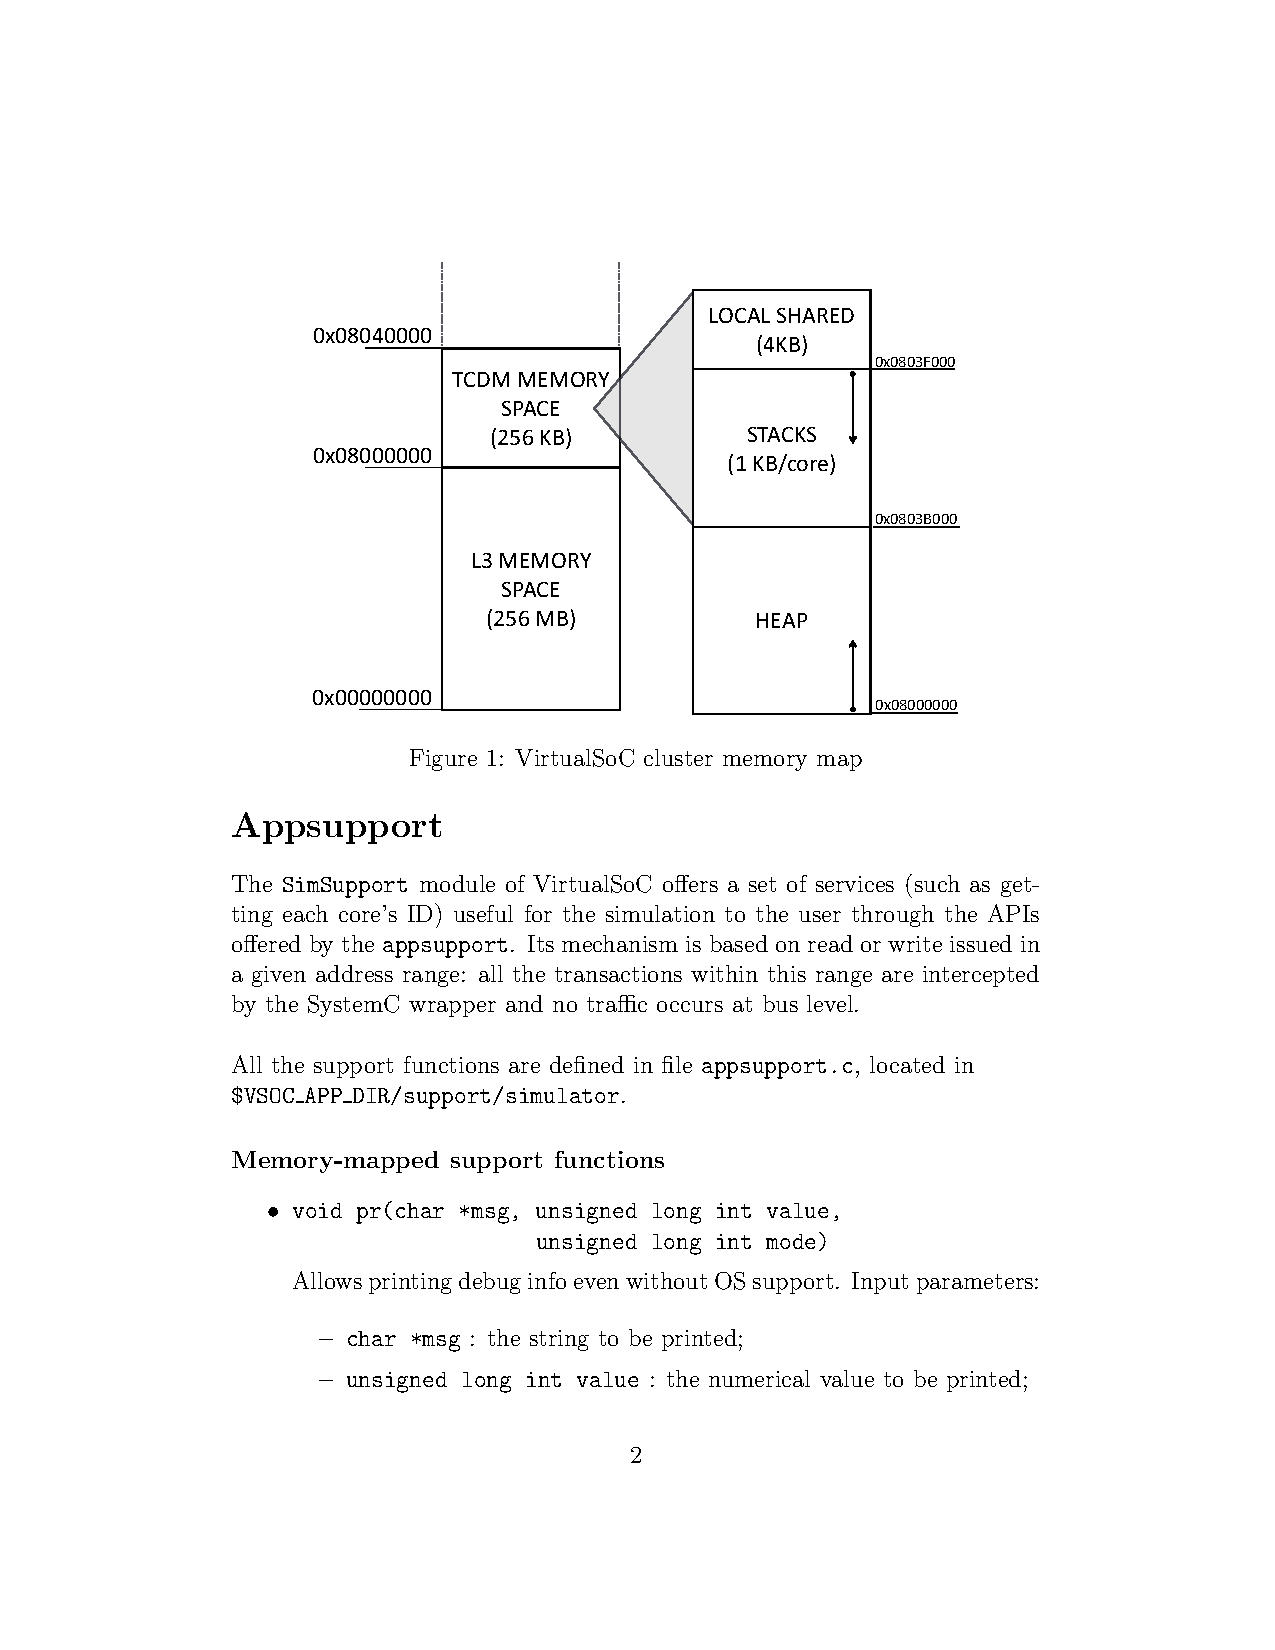
\includegraphics[trim = 50mm 155mm 50mm 40mm, clip, width=0.8\textwidth]{pictures/Memory_Architecture.pdf}
\end{center}

The picture above shows the memory architecture of VSoC. The lower end is filled by L3 memory (not supported yet), and TCDM comes right after it. TCDM is short for Tightly Coupled Data Memory. It's similar to a shared L1 cache, but with many banks. Each bank by itself supports memory and write, which means TCDM allows many memory accesses at the same time, as long as they belong to different banks. See  vsoc.pdf \cite{vsoc} for more details.

The TCDM memory space can be further divided into the stacks, the heap, and the local shared region. The heap is where we dynamically allocate memories, and the stack keeps track of local variables and function calls. It important to make sure that the heap and stack don't overlap. In other words, we should never allocate memory in the stack, otherwise we may get some weird errors. 

\subsection{Increase TCDM Size}
In VSoC, the default TCDM size is defined to be 0x40,000 Bytes (256 KB).  Unfortunately,  there are some particularly "hungary" applications that require more memory to run.  If we run these applications with the default TCDM size, VSoC will run out of shared memory and crash.

To solve this problem, we will need to increase the size of TCDM. Here is a step-by-step procedure:

\vspace{2mm}

1). Open vsoc-beta/src/core/config.h , and change CL\_TCDM\_SIZE (around line 60) to the desired value.

{
\addtolength{\leftskip}{6mm}

\vspace{-2mm}

\begin{itemize}
\item Skiplist on a 8-core system needs 0x00080000 Bytes (512KB) to run.
\item Skiplist on a 16-core system needs 0x000b0000 Bytes (768KB).
\item RedBlack on a 16-core system needs 0x00080000 Bytes (512KB).
\item Full version of Patricia needs 0x00400000 Bytes (4MB).
\end{itemize}

\vspace{-2mm}
See Sections 3.3.5, 3.3.6, and 3.3.7 for more details.

}

\vspace{2mm}
2). Open vsoc-beta/apps/support/simulator/vsoc.ld 

{
\addtolength{\leftskip}{6mm}

Change the value of STACK\_TOP (line 6) to 0x08000000 + CL\_TCDM\_SIZE - 0x1004.

Change the value of ORIGIN (line 10) to 0x08000000 + CL\_TCDM\_SIZE - 0x1000.

For example, if CL\_TCDM\_SIZE is set to be 0x00080000, then STACK\_TOP should be 0x0807effc, and ORIGIN should be 0x0807f000.

The variables STACK\_TOP and ORIGIN define the start of the stack. They need to change together with TCDM size to make sure that the stack is always located at the end of shared memory. See Section 2.1 for more details.

}

\vspace{2mm}
3). Go to the vsoc-beta directory, and run the following command:

{
\addtolength{\leftskip}{6mm}

\hspace{5mm}\texttt{\$ source SOURCEME}

}

\vspace{2mm}
4). Go to the vosc-beta/scripts directory, and run:

{
\addtolength{\leftskip}{6mm}

\hspace{5mm}\texttt{\$ vsoc\_clean}

\hspace{5mm}\texttt{\$ vsoc\_build -a}

}

\vspace{2mm}
5). Clean and recompile the benchmark (to make changes in vsoc.ld effective), and run it on the simulator.

\newpage
%----------------------------------------------------------------------------------------
%	Application Support
%----------------------------------------------------------------------------------------

\section{Application Support}

\subsection{Shared Memory Allocation}
\subsection{Initialization Flags}
\subsection{Global Pointers}
\subsection{Shared Memory Allocation}
\subsection{Barriers}
\subsection{Locks}

%----------------------------------------------------------------------------------------
%	Benchmarks
%----------------------------------------------------------------------------------------
\newpage
\section{Benchmarks}
\subsection{Compilation}

In order to compile each of the benchmarks, configure the Makefile to fit the system that you 
are running on. Check the environment variables and the compiler. If the compilation of the 
benchmark fails because a particular environment is not set, you can either add lines to the 
\textbf{.bashrc} file which will load the variables when a particular bash shell is initialized.  A sample section 
from our \textbf{.bashrc} file is shown below. Then run 
"make". This will create an executable binary file called \textbf{app.exe} in \textbf{o-optimize/} which is then 
made into 4 TargetMem\*.mem files in the main application directory. These are 
fed into the simulator when the benchmark is run. 

\bashscript{bash}{Sample .bashrc file for environment variables}

\subsection{Execution}

To run the benchmark on the simulator, the simulator first needs to know which 
benchmark you want to run. Move into the v\textbf{soc-beta/bin/} directory and run 
\textbf{vsoc\_set\_app}, which will provide a dialog in which you can choose a 
benchmark as the application that you want to run.  Make sure to choose 1 
binary for each cluster you would like to run (these benchmarks have only been 
tested with 1 cluster and 16 cores). When this script finishes, you can run the 
main VSoC simulator with a few runtime options. More information on these 
options can be found in the documentation for VSoC, found in \textbf{doc/}.  
A sample execution command would be:
\begin{center}
\begin{verbatim} 
	./vsoc.x -c16 --intc=c 
\end{verbatim} 
\end{center}
which would run a benchmark with 16 cores and 1 cluster. 

\subsection{Summaries}
\subsubsection{Hello World}

This benchmark simply prints out a "Hello World" statement to the screen. It 
was included in the version of VSoC that we downloaded and consisted of one 
line of code that printed a line of code to the screen. 

In the summer of 2013, Peng and Callen (Swarthmore College) made a few changes 
to the benchmark to test two of the application support functions that we made. 

\subsubsection{Count}

Count is a very basic benchmark that was obtained from Iris Bahar's Low Power 
VLSI System Design class at Brown University. The benchmark is included as an 
example in a shared memory synchronization lab for the class. It originally 
ran on the MPARM hardware simulator. Students are shown the unparallelized and 
the parallelized versions of the benchmark and then asked to perform similar 
modifications to another application. 

In the summer of 2013, we decided to port the benchmark from this lab 
application on MPARM to the VSoC system we were working on.  It was useful as 
a simple test of the locks implemented in VSoC (it turned out that these locks 
were not completely functional).

The functionality of the benchmark is simple. The cores take turns acquiring a 
lock for a shared counter. They increase it by one and release the lock. The 
final value of the counter is correct if none of the cores have interfered 
with each other's atomic increases.

\subsubsection{Matrix Multiplication}

Along with hello world, matrix mult is a benchmark that came with the VSoC 
system from University of Bologna. 

The operation of the benchmark is the multiplication of two arrays. These 
arrays are defined in matrix.h. Originally they were generated with MatLab and 
are sized 16x16. 

Matrix multiplication isn't terribly useful for synchronization tests because 
the application can simply break up the matrix into pieces and assign each 
core to have their own chunk.  They can store a local copy of the arrays and 
only operate on the part they are assigned to. Since this arrangement doesn't 
use locks, the matrix multiplication benchmark is more useful as a test of the 
VSoC installation but not in the testing of transactional memory. 

\subsubsection{C5}

The C benchmark was developed as a microbenchmark was developed by the team
from Brown University, Swarthmore College, and University of Bologna in 
transactional memory research. It utilizes basic synchronization on a scale 
much smaller than that of the STAMP benchmarks or even a benchmark like 
patricia.

The benchmark functions by performing operations on shared and local arrays. 
These operations are simple integer manipulation, and have no practical 
relevance. 

These operations are split into 4 parts in the C benchmark. Each core has a 
local array and there is also an array shared by all the cores. The local 
array just simulates work that doesn't require synchronization functionality. 
The shared array contains several vectors that overlap on each other. 
Constants such as the size of the vectors, number of overlap elements, and 
number of iterations performed are defined at the beginning of the testbench
 file. 

The locks required for the C benchmark are specifically assigned to certain 
areas of the array. The layout for the lock setup is shown in the main source 
file.

\subsubsection{Patricia}

The original patricia benchmark was written by Matt Smart from The University of
 Michigan. His description of the functionality of the program is provided
below:

\begin{verbatim}
    This code is an example of how to use the Patricia trie library for
    doing longest-prefix matching.  We begin by adding a default
    route/default node as the head of the Patricia trie.  This will become
    an initialization functin (pat_init) in the future.  We then read in a
    set of IPv4 addresses and network masks from "pat_test.txt" and insert
    them into the Patricia trie.  I haven't yet added example of searching
    and removing nodes.
\end{verbatim}

This version of Patricia was then ported to the MPARM system simulator used at 
the Univeristy of Bologna in research of Transactional Memory Systems. This
benchmark is useful because it contains several critical sections of code. 
Researchers can test different memory configurations in muti-core and many-core 
systems using the patricia benchmark because all the cores will have to share a 
single data structure. 

Finally, in the summer of 2013, Peng and Callen (Swarthmore College) ported 
thisbenchmark to the Virtual System on Chip (VSoC) simulator used by Brown 
University and Swarthmore College in transactional memory research for 
many-core clustered systems. 

\vspace{2mm}
\emph{*Important:} 

We reduced the input buffer size in this version of Patricia, because VSoC's default TCDM size doesn't support large input buffers. 

The input buffer size in Patricia is defined by two variables: INITSIZE, which is the number of nodes we pre-populate in the patricia trie, and BUFSIZE, the number of IP addresses we lookup and insert in the tree. Larger input buffer leads to a larger Patricia trie, which in turn needs more memory to allocate. The Patricia benchmark in MPARM had INITISIZE = 1024, and BUFSIZE = 4096. However, this specification needs a 4MB TCDM to run, while the default TCDM size is only 256KB. 

There are two solutions to this problem. We could reduce the input buffer size. If we decrease INITSIZE to 128, and BUFSIZE to 512, then Patricia runs well on VSoC. We could also increase the size of TCDM. See section 1.5 for more details.

\subsubsection{Skiplist}

The original skiplist benchmark was published on http://epaperpress.com
as a sorting and searching example. The descriptions can be found here:

http://epaperpress.com/sortsearch/skl.html

This version of skiplist was then ported to the MPARM system simulator used at 
the Univeristy of Bologna in research of Transactional Memory Systems. This
benchmark is useful because it contains several critical sections of code. 
Researchers can test different memory configurations in muti-core and 
many-core systems using the patricia benchmark because all the cores will have 
to share a single data structure. 

Finally, in the summer of 2013, Peng and Callen (Swarthmore College) ported 
thisbenchmark to the Virtual System on Chip (VSoC) simulator used by Brown 
University and Swarthmore College in transactional memory research for 
many-core clustered systems. 

\vspace{2mm}
\emph{*Important:} 

In this benchmark, every core has a privite skiplist, and together they have a
shared skiplist. Every skiplist needs 0x9010 bytes of shared memory, which 
means the 8-core version needs 0x9010 * (8+1) = 0x51090 bytes,
and the 16-core version needs 0x9010 * (16+1) = 0x99110 bytes. However, the 
default TCDM size in VSoC is only 0x40000 bytes. So we need to 
increase the TCDM size in order to run skiplist on 8 or 16 cores.
 See section 1.5 for more details.

There are also some parameters need to be set inside the benchmark, including 
 PERCENT\_LOOKUP, PERCENT\_INSERT, and PERCENT\_DELETE. They 
represent the percentage of lookup, insert, and delete operations to perform.
The default values are lookup = 90\%, insert = 9\%, and 
delete = 1\%. They can be found and set at the beginning of testbench.c,
and their values will affect the size of critical sections. 

\subsubsection{Redblack}


The original redblack benchmark was published on http://epaperpress.com
as a sorting and searching example. The descriptions can be found here:

http://epaperpress.com/sortsearch/skl.html

This version of redblack was then ported to the MPARM system simulator used at 
the Univeristy of Bologna in research of Transactional Memory Systems. This
benchmark is useful because it contains several critical sections of code. 
Researchers can test different memory configurations in muti-core and many-core 
systems using the patricia benchmark because all the cores will have to share a 
single data structure. 

\vspace{2mm}
\emph{*Important:} 

In this benchmark, every core has a privite redblack tree, and together they 
have a shared redblack tree. Every redblack tree needs 0x5010 bytes of shared 
memory, which means the 16-core version needs 0x5010 * (16+1) = 0x55110 bytes. 
However, the default TCDM size is only 0x40000 bytes. 
So we need to increase the TCDM size in order to run redblack on 16 cores. 
See section 1.5 for more details.

There are also some parameters need to be set inside the benchmark, including 
 PERCENT\_LOOKUP, PERCENT\_INSERT, and PERCENT\_DELETE. They 
represent the percentage of lookup, insert, and delete operations to perform.
The default values are lookup = 90\%, insert = 9\%, and 
delete = 1\%. They can be found and set at the beginning of testbench.c,
and their values will affect the size of critical sections. 


\subsubsection{K-Means}

K-means was originally included in Stanford's STAMP benchmark suite for 
multiprocessor systems.  It was then ported to the MPARM simulator, and this
file documents the changes necessary to run it on the VSoC simulator developed
by researchers from the University of Bologna. 

K-means is a clustering algorithms that can cluster a set of vectors into a 
certain number of groups.  For example, the main input to the benchmark
contains 64 vectors with 8 elements each. The system clusters them into 8
groups.  The test input, found in "goldinput.h", uses 12 objects each with 
2 attributes, and clusters them into 2 groups. 

The algorithm works in two stages. First, random vecors are chosen from the
set as the initial cluster centroids. Then, each vector is assigned to the 
centroid that is closest to it. The centroid is then recomputed as the point
which minimized the sum of squares distance between the centroid and each of 
the vectors. Then the vectors are reassigned again. These two steps are
iterated until no vectors switch centroids and the distance each centroid moves
when it is recalculated is reduced to zero. 

\subsubsection{Vacation}

Vacation was originally released as part of the STAMP benchmark suite. It was
ported to MPARM in the summer of 2008 by Trilok Acharya.

From the original README, 

\begin{verbatim}
    This benchmark implements a travel reservation system powered by a
    non-distributed database. The workload consists of several client threads
    interacting with the database via the system's transaction manager.

    The database is consists of four tables: cars, rooms, flights, and 
    customers. The first three have relations with fields representing a 
    unique ID number, reserved quantity, total available quantity, and price. 
    The table of customers tracks the reservations made by each customer and 
    the total price of the reservations they made. The tables are implemented 
    as Red-Black trees."
\end{verbatim}

It would be wise to read Trilok's README, found in the app directory, for 
details on how he ported the original STAMP benchmark to MPARM. In this README,
I will only discuss changes that were made by Peng and I to get the benchmark
to run on VSoC. The initial port to MPARM was a much, much larger project. 

\subsubsection{Genome}

The original genome benchmark was written by Chi Cao Minh from Stanford 
University. His description of the functionality of the program is provided 
below.

\begin{verbatim}
    This benchmark implements a gene sequencing program that reconstructs the 
    gene sequence from segments of a larger gene.

    For example, given the segments TCGG, GCAG, ATCG, CAGC, and GATC, the 
    program will try to construct the shortest gene that can be made from them.

    For example, if we slide around the above segments we can get:

             TCGG
        GCAG
            ATCG
      CAGC
           GATC
     =============
      CAGCAGATCGG

    This gives a final sequence of length 11. Another possible solution is:

        TCGG
           GCAG
       ATCG
            CAGC
      GATC
     =============
      GATCGGCAGC

    This solution has length 10. Both are consistent with the segments provided,
    but the second is the optimal solution since it is shorter.

    The algorithm used to sequence the gene has three phases:

        1) Remove duplicate segments by using hash-set
        2) Match segments using Rabin-Karp string search algorithm [3]
            - Cycles are prevented by tracking starts/ends of matched chains
        3) Build sequence

    The first two steps make up the bulk of the execution time and are 
    parallelized.


    References
    ----------

    [1] C. Cao Minh, J. Chung, C. Kozyrakis, and K. Olukotun. STAMP: Stanford 
          Transactional Applications for Multi-processing. In IISWC '08: 
          Proceedings of The IEEE International Symposium on Workload 
          Characterization, September 2008. 

    [2] C. Cao Minh, M. Trautmann, J. Chung, A. McDonald, N. Bronson, J. Casper,
          C. Kozyrakis, and K. Olukotun. An Effective Hybrid Transactional Memory
          System with Strong Isolation Guarantees. In Proceedings of the 34th 
          Annual International Symposium on Computer Architecture, 2007.

    [3] R. M. Karp and M. O. Rabin. Efficient randomized pattern-matching
         algorithms. IBM Journal of Research and Development, 1987.

\end{verbatim}

\subsubsection{Labyrinth}

The original labyrinth benchmark was written by Chi Cao Minh from Stanford 
University. His description of the functionality of the program is provided 
below.

\begin{verbatim}
    Given a maze, this benchmark finds the shortest-distance paths between
    pairs of starting and ending points. The routing algorithm used is Lee's 
    algorithm [2].
 
    In this algorithm, the maze is represented as a grid, where each grid 
    point can contain connections to adjacent, non-diagonal grid points. 
    The algorithm searches for a shortest path between the start and end 
    points of a connection by performing a breadth-first search and labeling 
    each grid point with its distance from the start. This expansion phase 
    will eventually reach the end point if a connection is possible. A second 
    traceback phase then forms the connection by following any path with a 
    decreasing distance. This algorithm is guaranteed to find the shortest 
    path between a start and end point; however, when multiple paths are made, 
    one path may block another.

    When creating the transactional version of this program, the techniques
    described in [3] were used. When using this benchmark, please cite [1].


    References
    ----------

    [1] C. Cao Minh, J. Chung, C. Kozyrakis, and K. Olukotun. STAMP: 
        Stanford Transactional Applications for Multi-processing. In IISWC
        '08: Proceedings of The IEEE International Symposium on Workload 
        Characterization, September 2008. 

    [2] C. Lee. An algorithm for path connections and its applications. IRE 
        Trans. On Electronic Computers, 1961.

    [3] I. Watson, C. Kirkham, and M. Lujan. A Study of a Transactional 
        Parallel Routing Algorithm. Proceedings of the 16th International 
        Conference on Parallel Architectures and Compilation Techniques, 
        2007.
\end{verbatim}

\subsubsection{ScalParC}


\newpage
\begin{thebibliography}{1}

\bibitem{vsoc} Daniele Bortolotti {\em vsoc-beta/doc/vsoc.pdf}, \hspace{2mm} VSoC beta release.

\bibitem{appsupport} MicrelLab - DEI {\em  vsoc-beta/doc/appsupport.pdf}, \hspace{2mm}  VSoC beta release.

\bibitem{setup} MicrelLab - DEI {\em  vsoc-beta/doc/setup.pdf}, \hspace{2mm}  VSoC beta release.

\bibitem{simulator} MicrelLab - DEI {\em  vsoc-beta/doc/simulator.pdf}, \hspace{2mm}  VSoC beta release.

\end{thebibliography}


%----------------------------------------------------------------------------------------

\end{document}